%%%%%%%%%%%%%%%%%%%%%%%%%%%%%% -*- Mode: Latex -*- %%%%%%%%%%%%%%%%%%%%%%%%%%%%
%% project.tex -- 
%% Author          : Philip Johnson
%% Created On      : Tue Nov  4 10:26:48 1997
%% Last Modified By: Philip M. Johnson
%% Last Modified On: Fri Jun 17 10:53:04 2005
%% RCS: $Id$
%%%%%%%%%%%%%%%%%%%%%%%%%%%%%%%%%%%%%%%%%%%%%%%%%%%%%%%%%%%%%%%%%%%%%%%%%%%%%%%
%%   Copyright (C) 1997 Philip Johnson
%%%%%%%%%%%%%%%%%%%%%%%%%%%%%%%%%%%%%%%%%%%%%%%%%%%%%%%%%%%%%%%%%%%%%%%%%%%%%%%
%% 

\section{Overview}

\subsection{Motivation}
As with baseball, physics, music, and other skillful human endeavours, there
is a vast range of ability associated with software development.  For
almost 40 years, software development researchers have been attempting to
understand, measure, and support the development of superior skill in
software development.  Sackman performed the seminal research on programmer
productivity in 1967, in which he reported a 28:1 difference between the
slowest and fastest programmers on a programming task \cite{Sackman68}.
Subsequent research by Prechelt on Sackman's original dataset in
combination with other published datasets indicates a smaller but still
significant multiple---from 2:1 to 6:1 depending upon conditions and the
kind of statistical comparison used \cite{Prechelt99}.  There is even 
evidence that some programmers may actually decrease overall productivity, 
a phenomenon known as the ``net negative producing programmer'' \cite{Schulmeyer92}.

While comparison of different individual's effort on a common programming task is the
most direct way to measure productivity variability, it is not the only way.
One alternative  employs the COCOMO II cost estimation model
\cite{Boehm00}. COCOMO uses a dataset of approximately 160 completed
industrial projects to calibrate a model that computes the effort required
to complete a project based upon characteristics of the software to be
developed and the organization doing the development.  In the COCOMO model, the
effort differential between best and worst programming teams with respect
to capability is 3.53, applications experience is 1.51, language and tools
experience is 1.43, platform experience is 1.40, and team cohesion is 1.29.
Multiply these together, and the COCOMO model indicates a theoretical
productivity difference of 13:1 between the most suited and least suited
programming teams for a given software project. 

%% Of course, one can also argue that there is infinite variability between
%% programmers, since certain kinds of programming tasks are so challenging
%% that some programmers will never complete them no matter how much effort
%% they invest. For example, in a private correspondence with a former member
%% of a tool development team for a major vendor, he stated that he viewed his
%% product as inferior to a competitor's and that it would most likely would
%% remain so regardless of the level of resources expended by his company,
%% basically because the competitor's product development was led by a world
%% class designer.  In summary, while the actual multiple can be debated, the
%% presence of substantial programmer variability cannot.

Programmer variability creates two basic kinds of challenges for the
software engineering research community: (1) How can we raise the average
productivity of software developers, and (2) How can we reduce the
variability between the best and worst software developers?  In general, we
have responded to these challenges in one or more of three ways: through
abstraction, automation, and through best practices.

The evolution of programming languages from machine language to assembly
language to high level languages to executable specification languages
exemplifies the successful use of abstraction to improve programmer
productivity by reducing the amount and complexity of code required to
accomplish a given task.  A single keyword such as ``synchronized'' in a
high level language like Java might require thousands of lines of code to
implement correctly in assembly language.  Indeed, software disasters such
as the Therac-25 were ultimately attributed to incorrect implementation of
process synchronization in application-level software \cite{Leveson93}.

Automation refers to the development of scripts or other approaches to
ensure that a sequence of development tasks are carried out consistently,
reliably, and correctly.  One example is an automated daily build
mechanism, which might (a) create a ``clean'' initial build state, (b)
check out the latest version of a system from a configuration management
repository, (c) compile the latest version, (d) deploy the latest version
to a run-time environment (such as installation on a web server), (e) run
all functional (i.e. unit) and non-functional (i.e. load) tests associated
with the latest version, (g) build the documentation associated with the
latest version, (h) generate a report associated with the build process,
and (i) email results to developers and managers.  

The difference between abstraction and automation is that abstraction
creates a ``black box'' for developers while automation does not. For
example, the implementation of the synchronized keyword in Java is a black
box: no application developer would be expected to maintain or debug this
language construct and, in general, developers simply assume that this
abstraction functions correctly.  A daily build script, however, is
typically designed, implemented, and maintained by developers, and thus
does not provide abstraction even though it does provide many benefits as a
form of automation. For example, it can eliminate the negative productivity
impact of developers not carrying out the sequence of actions required to
build the product correctly, or even not building the system at all due to
the time, overhead, and tedium associated with the activities.

While abstraction is the province of languages and other expressive media,
and automation is the province of tools and environments, best practices
unifies them with the behavior and activities of people during software development.
The seminal software engineering best practice is the waterfall lifecycle
model, which was first described in the early 1970's and provided an
efficient and effective partitioning of development into a sequence of
phases: specification, design, implementation, testing, and maintenance.
Provided that system requirements can be specified in advance and are
guaranteed not to change, the waterfall lifecycle model still constitutes a
viable best practice for software engineering.

The Software Engineering Body of Knowledge (SWEBOK) illustrates the variety
present in the best practices associated with our discipline
\cite{Abran05}.  SWEBOK provides a map to the state of the art in software
engineering, and divides the landscape into ten areas: requirements,
design, construction, testing, maintenance, engineering management,
configuration management, process, tools, and quality.  SWEBOK shows that
abstraction, automation, and best practices are not independent concepts
but are instead deeply entwined: best practices (such as testing) engender
new forms of abstraction (formal languages for testing) and automation
(tools for automated test definition and/or invocation). Conversely, new
tools (such as automated test frameworks) can catalyze new best practices
(such as test driven design).

One might naively assume that becoming a world class software developer
would require nothing more than downloading the SWEBOK and implementing all
of its best practices and their associated abstractions and automation.
Unfortunately, software engineering best practices are highly contextual: a
practice that provides immense benefits in one organizational culture and
development context might prove disastrous in another. For example, a best
practice such as Cleanroom might be essential in the development of a
complex, life-critical application but too time-consuming in a startup
environment where time to market is critical.  Furthermore, software
engineering best practices can be in conflict.  The Extreme Programming
\cite{Beck00} best practice eschews the use of the Code Inspection
\cite{Fagan76} best practice, claiming that the use of Pair Programming
obviates the need for a separate inspection activity.

The context sensitivity of software engineering best practices creates a
number of problems. First, how can an organization improve by adoption of
best practices when it is so difficult to determine their appropriateness?
Some organizations address this problem via a trial-and-error
approach, where various best practices are ``tried on for size''.  Others
hire consultants to tell the organization which practices to
adopt. Still others utilize models for process improvement such as
the CMMI \cite{Royce02}, which could be viewed as ``best practices for
adopting best practices''.

Second, how do ``best practices'' actually become recognized as such?  For
example, the best practice of ``Extreme Programming'' would have likely 
become a forgotten experiment in an alternative software development
process at Chrysler Corporation had Kent Beck not decided to vigorously
market the approach with books, lectures, and networking.  Ironically, the
project on which XP based its initial claims for success was eventually
cancelled without fulfilling its requirements and is now used as evidence
against XP by its detractors \cite{Keefer03}.

In summary, software engineering uses three methods to address the problem
of programmer productivity variability: abstraction, automation, and best
practices.  Unfortunately, the creation of best practices with the
abstraction and automation they require, and their adoption into new
contexts is traditionally mediated by political and social processes that
may be quite unrelated to the actual effectiveness of the practice and its
associated abstractions/automations in the organization.


\subsection{Approach}

This research proposal presents a new, continuous, evidence-based approach
to the generation and adoption of best practices.  Instead of looking
outward into the community for best practices, and attempting to adapt them
to one's own environment, our research will investigate how best practices
can be identified and evaluated within one's current organizational and
project context.  Instead of relying on politics or persuasiveness for
adoption, our research involves instrumentation that continuously generates
empirical data as evidence either for or against the suitability of a
practice.  Finally, our research will involve adaptation of data mining
approaches to support the discovery of candidate best practices from
software engineering process and product data.

This research approach leverages our research and development activities
over the past four years in Project Hackystat \cite{Hackystat}, an open
source framework for continuous, automated collection and analysis of
software engineering process and product data.  Hackystat implements an
automated approach to metrics collection by attaching sensors to
development tools. This makes it possible to capture both low and
high-level data about processes and products with a combination of
precision, completeness, and low overhead not possible with manual
approaches. Hackystat also provides a robust implementation of Software
Project Telemetry, an approach to in-process monitoring, analysis, and
decision-making based upon the generation of high-level abstractions of the
sensor data stream.  Software Project Telemetry provides a means to
understand whether measures of process and produce are stable, improving,
or declining over a particular interval in time. Finally, Hackystat
provides a prototype implementation of Software Development Stream
Analysis, which observes the low-level behaviors of individuals as they
manipulate tools, abstractions, and automation, then classifies them as
indicating the use of a best practice.  For example, SDSA implements
techniques to identify when a developer is using the ``test-driven design''
best practice.

The combination of Hackystat, Software Project Telemetry, and Software
Development Stream Analysis provide a mechanism for continuous,
context-sensitive evaluation of best practices within an organization.  For
example, an organization using Hackystat on a project can use Software
Project Telemetry to establish baseline values for various software
development measures.  Software Development Stream Analysis provides a way
to identify the use of certain best practices by developers.  Integrating
these techniques provides a way to relate the practices of
developers to their outcomes in terms of process and product measures. 
For example, if a development group decides to adopt the use of pair
programming on a trial basis, they can see if this new practice makes an
impact on the measures of process and product captured by Software Project
Telemetry.  Conversely, if Software Project Telemetry reveals a significant
decline in process or product metrics (such as a drop in the test case
coverage of the system), then Software Development Stream Analysis can be
used to assess whether some change in practice could be responsible (such
as a change from test-first to test-last design).

Hackystat, Software Project Telemetry, and Software Development Stream
Analysis together form an empirical, continuous, low-cost, and in-process
approach to assessing best practices when the practices are known a priori
and recognition rules for them can be built into the SDSA system.  An
additional component of this research will investigate approaches to the
discovery of new best practices.  To do this, we will incorporate recent
research in data mining for pattern discovery
\cite{Heierman04,Mannila95,Agrawal95}.  The goal of pattern discovery is to
uncover repeated behaviors in a stream of time-stamped data.  For example,
in a ``smart house'', if an occupant repeatedly turns on a light after
opening the front door, the pattern discovery mechanism should discover
this pattern after a number of repetitions, thus enabling the smart house
to begin automatically turning on the light whenever the front door is
opened by this occupant.  In this research, we will explore the use of
pattern discovery in combination with Software Project Telemetry to uncover
candidates for new ``best practice'' developer behaviors.  As a simple
example, pattern discovery might find that one developer consistently
writes and executes tests against their code prior to committing it to the
CVS repository. If Software Project Telemetry reveals that this pattern is
associated with significantly less daily build failures, then this pattern
is a candidate for a new ``best practice'' for this development group and
project.

Our approach compares in interesting ways to the more traditional approach
to evaluation of best practices.  Both approaches involve a trial adoption
of the best practice, the collection of data on the effect of the practice,
and an eventual assessment of efficacy of the practice. However, the
traditional approach typically involves a ``one off'' experiment on a
sample project with specialized data collection during the project, and
analysis of the success or failure of the practice once the project is
concluded.  In contrast, our approach involves the introduction of
sensor-based instrumentation into the development environment, which allows
continuous, in-process collection and analysis of data concerning the
practice.  This has two significant implications. First, the presence of
automated metrics collection and analysis allows for more ``opportunistic''
evaluation of new practices at any point in a project's lifecycle: there is
no need to create a special project with special instrumentation for
evaluation purposes. Second, the presence of instrumentation enables a
``bottom-up'' approach to best practice discovery, in which the behaviors
of successful practitioners can be analyzed for the presence of repeated
patterns, and compared to process and product-based measures to see if they
constitute candidate best practices.

\subsection{Objectives}
\label{sec:objectives}

The overall objective of this research is to design, implement, and
evaluate a continuous, evidence-based approach to in-process discovery and
assessment of context-sensitive best practices during software development.
This overall objective has seven sub-objectives:

\begin{itemize}
  
\item Enhancement of the Software Development Stream Analysis mechanism to
  support a variety of current best practices, and determination of the
  kinds of abstractions, automation, and best practices that are amenable
  to recognition using SDSA.

\item Development of integration mechanisms between SDSA and Software
  Project Telemetry in order to allow users to determine how practices
  recognized by SDSA relate to telemetry data at any particular point in time.
  
\item Development of a pattern discovery subsystem in Hackystat to support
automated recognition of behavioral patterns by developers as they use tools, 
abstractions, and automation, and the use of Software Project Telemetry to 
determine whether these behavioral patterns are potential candidates for best
practices. 
  
\item Classroom-based, case study evaluation of the proposed techniques. We will 
apply these techniques to gain evidence regarding programmer productivity and variability 
with respect to the Test Driven Design best practice. This activity will also 
refine the technology, develop curriculum materials, and ready the approach for 
industrial evaluation. 

\item Industry-based evaluation of the proposed techniques. Following
classroom evaluation, we will carry out two industry-based case studies
to gather evidence regarding best practices related to high performance computing 
and agile software development. This activity will also assess our approach
in industrial settings. 
  
\item Packaging of the system and methods for widespread dissemination.  We
will continue the process used by the open source Hackystat Project of making
our technology available to the software engineering community.  In addition, 
we will package and disseminate our experimental methods to support external
evidence-based software engineering efforts. 
  
\item Development of curriculum materials regarding continuous,
  evidence-based discovery and assessment of software engineering best
  practices. As with the Hackystat Project, we will develop software engineering
  curriculum materials and assignments that enable the study and analysis
  of this approach in academic settings.

\end{itemize}


\section{Related Work}

\subsection{Hackystat}

For the past several years, we have been developing a framework for
automated software development process and product metric collection and
analysis called Hackystat.  This framework differs from other approaches to
software product and process measurement in one or more of the following ways:

\begin{itemize}

\item Hackystat uses sensors to unobtrusively collect data from development
environment tools; there is no chronic overhead on developers to collect
product and process data.  In contrast, tools such as the Process Dashboard
\cite{PSPDashboard} involve manual data collection. 

\item Hackystat is tool, environment, process, and application agnostic.
The architecture does not suppose a specific operating system platform, a
specific integrated development environment, a specific software process,
or specific application area.  A Hackystat system is configured from a set
of modules that determine what tools are supported, what data is collected,
and what analyses are run on this data. In contrast, tools such as TSP Tool
\cite{TSPTool} implement support for a fixed set of metrics under a fixed
process on a single platform.

\item Hackystat is intended to provide in-process project management
support. Traditional software metrics approaches, such as 
the NASA Metrics Data Program \cite{MDPRepository},  are based upon the
``project repository" method, in which data from prior completed projects
are used to make predictions about a future
project. In contrast, Hackystat is designed to continuously collect data from a current,
ongoing project, and use that data as feedback into the current project.

\item Hackystat is open source and is available to the academic and
commercial software development community for no charge. In contrast,
commercial toolkits such as MetricCenter \cite{MetricCenter} are closed
source and require licensing fees.

\end{itemize}

The design of Hackystat \cite{csdl2-02-07} reflects prior 
research in our lab on software measurement, beginning with research into
data quality problems with the PSP \cite{csdl-98-11} and continuing with
research on the LEAP system for lightweight, empirical, anti-measurement
dysfunction, and portable software measurement \cite{csdl2-00-03}.

\begin{figure*}[ht]
  \centering
  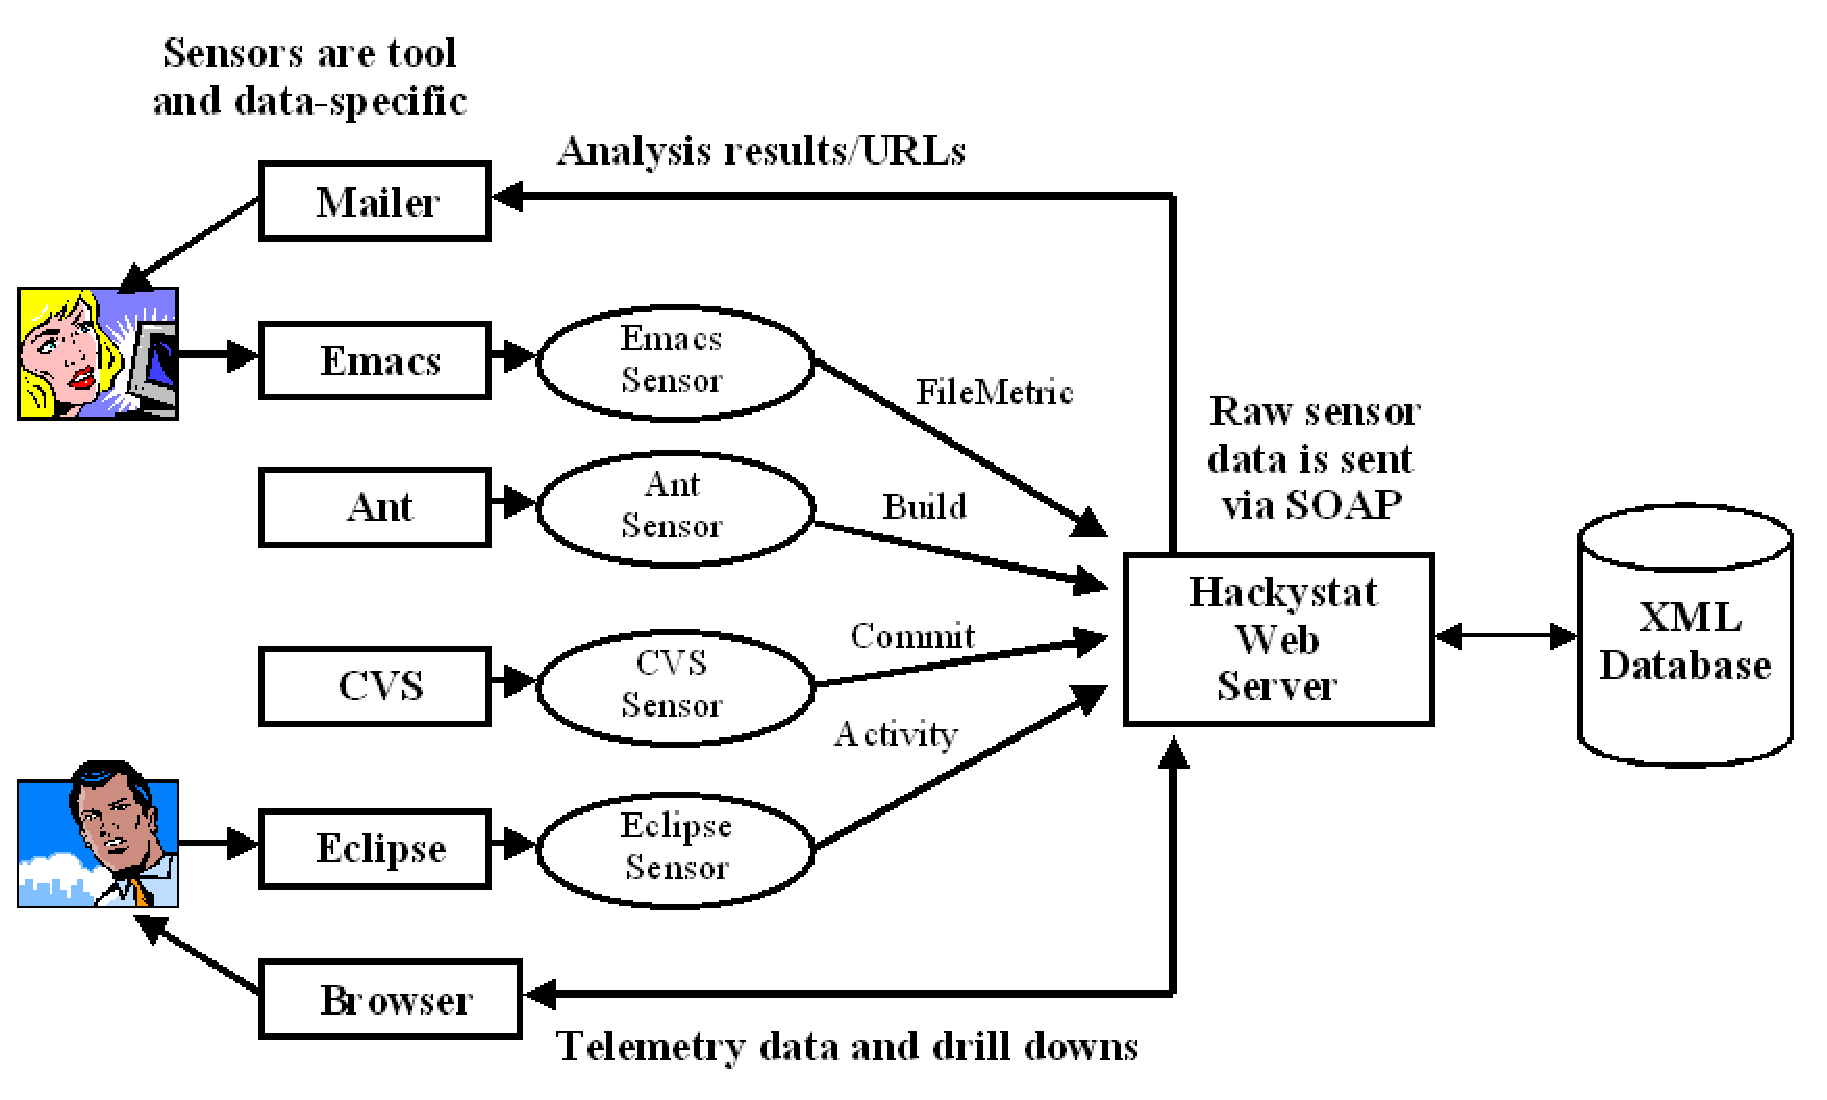
\includegraphics[width=0.60\textwidth]{architecture.eps}
  \caption{The basic architecture of Hackystat. Sensors are attached to
  tools directly invoked by developers (such as Eclipse or Emacs) as
  well as to tools implicitly manipulated by developers (such as CVS or 
  an automated build process using Ant).}
  \label{fig:architecture}
\end{figure*}

To use Hackystat, the project development environment is 
instrumented by installing Hackystat sensors, which developers attach
to the various tools such as their editor, build system, configuration
management system, and so forth. Once installed, the Hackystat sensors
unobtrusively monitor development activities and send process and
product data to a centralized web server.  If a user is working
offline, sensor data is written to a local log file to be sent
when connectivity can be re-established.
Project members can log in to the web server to see the collected
raw data and run analyses that integrate and abstract the raw sensor
data streams into telemetry.  Hackystat also allows project members to
configure ``alerts`` that watch for specific conditions in the
sensor data stream and send email when these conditions occur. Figure
\ref{fig:architecture} illustrates the basic architecture of the system. 

Hackystat is an open source project. Its sources, binaries, and
documentation are freely available online.  We also maintain a public
server running the latest release of the system at
http://hackystat.ics.hawaii.edu.  Hackystat has been under active
development for approximately four years, and currently consists of
approximately 1500 classes and 95,000 lines of code.  Sensors are available
for a variety of tools including Eclipse, Emacs, JBuilder, Jupiter, Jira,
Visual Studio, Ant, JUnit, JBlanket, CCCC, DependencyFinder, Harvest, LOCC,
Office, and CVS.

Hackystat is being used in a variety of academic and industrial contexts.
At the University of Hawaii, Hackystat has been tightly integrated into the
undergraduate and graduate software engineering curriculum, and is
used by approximately 50 students per year to support project
development \cite{csdl2-03-12}.  A researcher from the Free University of
Bozen came to Hawaii to study the Hackystat system in support their research on
PROM \cite{Sillitti03}.  Researchers at the University of Maryland are
using Hackystat to support assessment of programmer effort
\cite{Hochstein05}.  Hackystat has been used at NASA's Jet Propulsion
Lab to analyze the daily build process for the Mission Data System
\cite{csdl2-03-07}.  Finally, Hackystat is being used at SUN Microsystems
to support research on high performance computing system development
productivity \cite{csdl2-04-03}.

\subsection {Software Project Telemetry}
\label{sec:telemetry}

The automated, unobtrusive, continuous, and low-cost measurement
infrastructure provided by Hackystat enabled us to develop a new approach
to software measurement analysis called ``Software Project Telemetry``. 
According to Encyclopedia Brittanica, telemetry is a ``highly automated
communications process by which measurements are made and other data
collected at remote or inaccessible points and transmitted to receiving
equipment for monitoring, display, and recording.''  We
define Software Project Telemetry as a style of software engineering
process and product collection and analysis which satisfies the following
five properties:

{\em (1) Software project telemetry data is collected automatically by tools
that unobtrusively monitor some form of state in the project development
environment.}  In other words, the software developers are working in a
``remote or inaccessible location'' from the perspective of metrics
collection activities. This contrasts with software metrics data that
requires human intervention or developer effort to collect, such as PSP/TSP
metrics \cite{Humphrey95}.
        
{\em (2) Software project telemetry data consists of a stream of
time-stamped events, where the time-stamp is significant for analysis.}
Software project telemetry data is thus focused on evolutionary processes
in development.  This contrasts, for example, with COCOMO \cite{Boehm00},
where the moment in time at which calibration data is collected is not
generally significant.

{\em (3) Software project telemetry data is continuously and immediately
available to both developers and managers.}  Telemetry data is not hidden
away in some obscure database guarded by the software quality improvement
group.  It is easily visible to all members of the project for
interpretation.

{\em (4) Software project telemetry exhibits graceful degradation.}  While
complete telemetry data provides the best support for project management,
the analyses should not be brittle: they should still provide value even if
sensor data occasionally ``drops out`` during the project. Telemetry
collection and analysis should provide decision-making value even if these
activities start midway through a project.
         
{\em (5) Software project telemetry is used for in-process monitoring, control,
and short-term prediction.} Telemetry analyses provide representations of
current project state and how it is changing at the time scales of days,
weeks, or months.  The simultaneous display of multiple project state
values and how they change over the same time periods allow opportunistic
analyses---the emergent knowledge that one state variable appears to
co-vary with another in the context of the current project.

Software Project Telemetry enables an incremental, distributed,
visible, and experiential approach to project decision-making. For example,
if one finds that complexity telemetry values are increasing, {\em and}
that defect density telemetry values are also increasing, then one could
try corrective action (such as simplification of overly complex modules)
and see if that results in a decrease in defect density telemetry
values. One can also monitor other telemetry data to see if such
simplification has unintended side-effects (such as performance
degradation).  Project management using telemetry thus involves cycles of
hypothesis generation (Does module complexity correlate with defect
density?), hypothesis testing (If I reduce module complexity, then will
defect density decrease?), and impact analysis (Do the process changes
required to reduce module complexity produce unintended side-effects?).
Finally, Software Project Telemetry supports decentralized project
management: since telemetry data is visible to all members of the project,
it enables all members of the project--developers and managers--to engage
in these management activities.  

\begin{figure*}[ht]
  \centering
  \includegraphics[width=0.75\textwidth]{BuildAndChurn.eps}
  \caption{This telemetry report shows how code churn (lines
  added and lines deleted) co-varies with build failures over a four month period.} 
  \label{fig:telemetryreport}
\end{figure*}

As a concrete example of telemetry, consider Figure
\ref{fig:telemetryreport}. This report illustrates the relationship between
aggregate code churn (the lines added and deleted from the CVS repository
by all members of the project) and the number of build failures
over a four month period on the Hackystat project. Note how closely these
two measures co-vary, even though one is a process measure (build failure)
and the other is a product measure (code churn).  From this initial
observation, one could investigate other time periods and time scales to
see if this relationship holds in other contexts, as well as test
hypotheses on how to reduce build failures or predict their impact on the
project schedule.

The computational path from the sensors in Figure \ref{fig:architecture} to the telemetry
report in Figure \ref{fig:telemetryreport} involves several steps.  In the
first step, ``raw'' sensor data is collected from small software plug-ins
attached to developer tools. For example, an editor sensor may record a
``state change'' event when a file has been edited within the last 30
seconds by the user.  A CVS sensor may record the number of lines added and
deleted from a file during the past 24 hours.  This raw data is sent from
the sensors to a Hackystat server, where they are persisted in an XML-based
repository.  In the second step, the system abstracts the raw sensor data
into one or more ``DailyProjectData'' instances, which synthesize raw
sensor data from multiple group members and/or multiple sensors into a
higher level abstraction.  For example, a DailyProjectData instance might
process low-level ``state change'' events from multiple developers and
determine the total amount of time spent editing files by all members of
the project group for a given day.  In the third step, special classes
called ``Reduction Functions'' manipulate DailyProjectData instances to
create the sequence of numerical telemetry values
associated with a given project and time interval. For example, a Reduction
Function might manipulate a set of DailyProjectData instances to produce a
sequence of numerical telemetry values indicating LOC/hour.

In one application of Software Project Telemetry, we are
creating telemetry streams to support diagnosis of daily build failures and
reduce the productivity impact of their occurrence over time
\cite{csdl2-04-11}.  Another application involves the development of
specialized telemetry streams for high performance computing software to
better understand the bottlenecks present in the development of those
systems \cite{csdl2-04-22}.

\subsection{Software Development Stream Analysis}

Software Project Telemetry supports a ``macro'' view of project
development; telemetry aggregates data over all of the developers in a
project and all of its artifacts at time scales of days, weeks, or months.
A more recent research effort of ours focuses on a ``micro'' view of
project development, in which we seek to analyze developer behaviors at the
time scale of minutes or hours and identify whether they constitute the use
of a best practice.  Our approach is called ``Software Development Stream
Analysis'' (SDSA).

For example, consider the best practice called ``test driven design'' (TDD)
\cite{Beck03}.  TDD is often explained through a stop light metaphor, which
cycles from green to yellow to red.  At the beginning of a TDD cycle, the
code is working, and the stop light is green.  The developer then defines a
new test case that tests a new (and as yet unimplemented) feature.  This
will produce a syntax (compilation) error because that feature is not even
implemented yet.  This changes the stop light to yellow.  Consequently, the
developer implements a stub version of the feature, which fixes the
compilation error but produces a test failure.  This changes the stop light
to red. Once the developer finishes implementing the feature, the light
changes to green and the cycle begins again.  The stop light metaphor is
interesting because out of sequence lights indicate violations of the TDD
development pattern; for example, green to red indicates that the developer
added new code without adding a test for it first.

The goal of Software Development Stream Analysis is to support automated
recognition of development practices such as TDD.  SDSA involves a four
step process. First, Hackystat sensors collect raw data sufficient to
allow identification of the development behavior of interest. In the case
of TDD, the sensor must collect editing events,
compilation events, test invocation events, and their results.  Once the
appropriate form of raw data is available, SDSA takes the raw event stream
and ``tokenizes'' it by replacing sequences of raw data representing one
type of behavior by a single token representing that behavior. For example,
if the user edits the same file for several minutes, several dozen ``state
change'' events may be generated in the raw data stream. The SDSA tokenizer
replaces these by a single ``Edit'' token. Once the raw data stream is
tokenized, SDSA partitions it into a set of episodes.  In the case of TDD,
a ``test pass'' event serves as the delimiter between episodes.  Finally, a
rule-based engine based upon JESS \cite{Friedman-Hill:03} processes each
episode and classifies its development behavior, or returns Unknown if the
episode does not fit any of the known behaviors.

\begin{figure*}[ht]
  \centering
  \includegraphics[width=0.75\textwidth]{sdsa.eps}
  \caption{SDSA classifies this episode as ``(TDD, 2)''. This represents a
normal TDD cycle.  The two shaded ``COMPILE'' cells are yellow, and the
last two ``UNIT TEST'' cells are red and green, respectively.}
  \label{fig:sdsa}
\end{figure*}

Figure \ref{fig:sdsa} illustrates the use of SDSA to classify developer
behavior as belonging to the TDD best practice. This screen image shows the
first episode of a programming session on March 15, 2005, whose total
duration was a little over three minutes.  In this episode, the developer
began by implementing a class named TestStack. He then attempted to compile
the class, but it failed to compile since the class it was testing (Stack)
was not implemented.  SDSA indicates this with a (yellow) Compile token.
The developer implements the Stack class, but forgets the isEmpty() method,
yielding another yellow Compile error. Finally, the Stack class stub is
implemented, producing a (red) Unit Test Failure token.  A short time
later, the remainder of the Stack class is implemented, producing a (green)
Unit Test Pass token, which completes the TDD episode.

Our research on SDSA is less mature than our research on Software Project
Telemetry, and we are only beginning the process of evaluating its
generality and utility.  Our initial pre-pilot experiments in the domain of
Test Driven Design appear promising, and the system has been able to
correctly classify TDD episodes with over 80\% accuracy in a small sample
of developer data.   Currently, Eclipse is the only development
environment for which we have developed a Hackystat sensor that captures
the kinds of raw sensor data required for TDD recognition. SDSA is currently 
focused on representation of a single developer's behavior, although we have
begun preliminary design work on representations of group practices. 

In this research, we propose to investigate the potential synergy between
Software Project Telemetry and Software Development Stream Analysis.
Software Project Telemetry provides an efficient and effective mechanism
for detecting changes in the measures describing a project.  With
telemetry, we can easily detect that test case coverage is going down, or
build failures are going up, or inter-package coupling is increasing, or
the variance in developer active time is decreasing. Telemetry can tell us
that project characteristics are changing, but offers no insights into the
behaviors that led to these changes.  SDSA provides the opposite: it gives
us insight into the behaviors that are occurring during development, but
does not tell us what the impact of these behaviors might be on the
project.

The integration of these two analysis mechanisms provides a powerful
vehicle for evidence-based investigation of software development best
practices.  In the case of test-driven development, its proponents have
made radical claims for the technique: that it produces 100\% test case
coverage, that it produces higher quality software, more maintainable
software, and improves programmer productivity.  Initial empirical studies
of TDD have not provided strong evidence for or against these claims
\cite{George:03,George:04,Geras:04,Muller:02,Matjaz:03}.  Using Hackystat,
Software Project Telemetry, and SDSA, we can provide a replicable, standard
infrastructure that automatically (a) gathers outcome measures, such as
coverage, active time, and unit test invocations; and (b) assesses
compliance with the definition of TDD, so that we know whether the
experimental subjects were actually using the technique without requiring
physical observation. We will discuss this research effort further in
Section \ref{sec:research-plan}.

\subsection{Pattern Discovery}

Recent research in knowledge discovery and data mining involves processing
time ordered input streams and discovering the most frequently recurring
patterns.  Much of this work is based upon the Rissanen's Minimum Description Length 
(MDL) principle \cite{Rissanen89}.  The basic idea of this principle is that 
any regularity in a given set of data can be used to compress the data.  The
more regularities there are, the more the data can be compressed, and the more 
confidence we have that this regularity represents a meaningful pattern in the data. 

Heierman and his colleagues created the ED (Episode Discovery) algorithm
\cite{Heierman04}, which is based upon MDL but provides enhancements to
support natural forms of periodicity in human-generated timestamp data.
For example, a person might log in to their computer every weekday morning
between 8:00am and 8:30am.  ED includes explicit support for representing
such periodicity in the description language, which results in shorter
representations for periodic patterns. In addition, and unlike SDSA, ED
does not require an apriori specification of how a time-ordered sequence is
partitioned into episodes, but determines them automatically.  Mannilla and
colleagues also developed an episode discovery algorithm that they applied
to the stream of events in a telecommunication network alarm log, with the
goal of better understanding the causes of alarms, to suppress redundant
alarms, and predict future faults \cite{Mannila95}.  
%% Finally, Cook and colleagues
%% performed some initial research on pattern discovery using algorithmic 
%% grammar inference, Markov models, and neural networks \cite{Cook98b}.

Pattern discovery techniques such as these appear to hold great promise for
application to the data collected by Hackystat sensors, which is
time-stamped, periodic, and may or may not have naturally occuring
``episode'' boundaries depending upon the purpose of the analysis.  Pattern
discovery can complement SDSA: once a pattern is found via Pattern
Discovery and validated as interesting, a set of SDSA rules can be
developed that represent the ``best practice'' represented by the pattern,
which might be more general than the original behaviors analyzed.

\subsection{Evidence-based software engineering}

A recent revolution in medical research involves the introduction of an
``evidence-based'' paradigm.  This paradigm arose in response to two
observations: the failure to organize medical research into systematic
reviews could cost lives, and the clinical judgement of experts compared
unfavorably with the results of systematic reviews.   The evidence-based 
approach is starting to be applied outside of medicine, in fields such as
psychiatry, nursing, social policy, education, and software engineering. 

Kitchenham has been leading the movement for evidence-based software
engineering, organizing workshops on this topic and publishing papers
explaining the issues involved in applying evidence-based research
techniques to software engineering \cite{Kitchenham04,Kitchenham04a}.  She
and her collaborators propose a five step method for evidence-based
software engineering: (1) Convert the need for information [about a
software engineering practice] into an answerable question; (2) Track down
the best evidence available for answering the question; (3) Critically
appraise that evidence using systematic review for its validity (closeness
to the truth), impact (size of the effect), and applicability (usefulness
in software development practice); (4) Integrate the critical appraisal
with current software engineering knowledge and stakeholder values [to
support decision-making]; (5) Evaluate the effectiveness and efficiency in
applying Steps 1-4 and seek ways to improve them for next time.  While
promising, application of systematic reviews and the integration of
empirical software engineering data from multiple sources has been found to
be challenging \cite{Jedlitschka04}.

Our proposed research is designed to provide technology, data, and
methodology to support evidence-based software engineering.  The Hackystat
framework, along with Software Project Telemetry, Software Development
Stream Analysis, and Pattern Discovery applications, provides new and useful
infrastructure for the creation of evidence regarding a given software
engineering practice. Our case studies in the classroom setting will create
new, replicable data that can be used in evidence-based evaluation of the
test-driven design, and our industrial case studies will provide similar
evidence for high performance computing productivity.  Finally, our
experiences applying the tools and analyzing the data will result in our
recommendations for effective ways to utilize the technologies and assess
the data that results.

\subsection{Results from prior NSF research}

\small
\begin{tabular}{lp{4.5in}}

Award number: & CCF02-34568 \\
Program: & Highly Dependable Computing and Communication Systems Research\\
Amount: & \$638,000 \\
Period of support: & September 2002 to September 2006 \\
Title of Project: & Supporting development of highly dependable software through
continuous, automated, in-process, and individualized software measurement validation \\
Principal Investigator: & Philip M. Johnson \\
Selected Publications: & \cite{csdl2-04-22,csdl2-04-13,csdl2-04-11,csdl2-03-12,
csdl2-02-07,csdl2-03-07,csdl2-04-02,csdl2-04-04,csdl2-04-06}
\end{tabular} \\ %[3mm]
\normalsize

\medskip

The general objective of this research project is to design, implement, and
validate software measures within a development infrastructure that
supports the development of highly dependable software systems.
Contributions of this research project include: (a) development of a
specialized configuration of Hackystat to automatically acquire build and
workflow data from the configuration management system for the Mission Data
System (MDS) project at Jet Propulsion Laboratory; (b) development of
analyses over MDS build and workflow data to support identification of
potential bottlenecks and process validation; (c) identification of
previous unknown variation within the MDS development process; (d)
development of a generalized approach to in-process, continuous measurement
validation called Software Project Telemetry, (e) substantial
enhancements to the open source Hackystat framework, improving its
generality and usability; (f) development of undergraduate and graduate
software engineering curriculum involving the use of Hackystat for
automated software engineering metrics collection and analysis; (g) support
for 3 Ph.D., 6 M.S., and 3 B.S. degree students. 

\section{Research Plan}
\label{sec:research-plan}

\subsection{Task descriptions}


Our research plan follows the detailed objectives for this research as
summarized in Section \ref{sec:objectives}, and consists of the following
seven tasks.

{\em (1) Enhancement of the Software Development Stream Analysis
mechanism.}  An initial task is to enhance our prototype SDSA
implementation with support for more types of sensor data, more interactive
development environments, and more kinds of developer
behaviors than test driven development.  Additional sensor data streams
include defect data reports, software complexity measures, and performance
analysis data.  Additional interactive development environments include
Emacs, NetBeans, and Visual Studio.  Additional developer behaviors include
configuration management commit behaviors, defect management behaviors, and
software review behaviors.  

{\em (2) Development of integration mechanisms between SDSA and Software
Project Telemetry.}  Currently, Hackystat does not provide any support for
relating the analyses of SDSA to those of Software Project Telemetry.  In
this task, we will develop such mechanisms.  In general, the goal is to
support the display of relationships in two directions. Given the
identification of an interesting SDSA behavior, we will display
potentially relevant telemetry streams in the period surrounding that
behavior.  Conversely, given the identification of an interesting change in
the telemetry associated with a given project, we will display the
SDSA behaviors in the period surrounding that change.

{\em (3) Development of a pattern discovery subsystem.}  This task
involves the design and implementation of a new analysis module in
Hackystat for pattern discovery.  We will begin by reimplementing published
algorithms, such as the ``episode discovery'' algorithm
\cite{Heierman04}. This algorithm is particularly interesting because it
does not require an apriori partitioning of the event stream into discrete
episodes for classification (as is currently the case for SDSA), but rather
identifies episodes as an intrinsic part of the pattern discovery process.
After implementing the algorithm, we will test it on a variety of data sets
in order to assess its utility and effectiveness. For example, can the analysis
``discover'' Test Driven Design when provided with a set of event
streams enacting this behavior?  

{\em (4) Classroom-based, case study evaluation of the proposed
techniques.}  Once we have implementations of SDSA, its Telemetry
integration, and Pattern Discovery, we will begin classroom studies to
assess their utility and effectiveness in classroom conditions.  Over the
past several years, we have integrated Hackystat into the undergraduate and
graduate software engineering curriculum at the University of Hawaii. Our
students now routinely install sensors, collect and analyze process
and product metrics, and use this data to guide project management
\cite{csdl2-03-12}.  This provides an excellent environment for evaluation
of new Hackystat-based technologies.

We plan to evaluate SDSA and Telemetry integration though a case study of
test-driven design with three experimental phases.  In the first phase at
the beginning of the course, we will introduce ``traditional'' unit testing
and have them carry out a project assignment that requires them to achieve
at least 90\% coverage (to guarantee a minimal level of test case quality)
but without specifying when or how to develop the test cases.  We will use
SDSA to verify that students are not using TDD for this phase, and use
Software Telemetry to assess coverage, LOC/Hour, and other indicators of
quality and productivity.

In the second phase of the experiment, we will introduce principles of TDD,
provide a short assignment for them to use to learn TDD, then have them
carry out a project assignment that requires both the use of TDD and at
least 90\% coverage. We will use SDSA to verify that the students are using
TDD during this project, and Software Telemetry to assess the same
indicators of quality and productivity as before.  We can compare the
values of these indicators to see if any changes occur from the
introduction of TDD. For example, does the introduction of the TDD best
practice improve average programming productivity?  Does it decrease the
variation in programmer productivity?

In the third phase of the experiment, we will have the students carry out a
final project assignment, and this time require 90\% coverage but allow
them to choose their test development process.  We will use SDSA to
determine what percentage of the students use TDD and how consistently they
use TDD. We will use telemetry to see how quality and productivity measures
have changed relative to earlier phases.

In all phases, we will be applying the pattern discovery mechanism to the 
behavioral data that we obtain, and testing to see if we can discover interesting
patterns and if they relate to the telemetry data in useful ways.  

At the end of the study, we will collect qualitative data using a questionnaire to
assess student attitudes towards Hackystat, TDD, SDSA, and pattern discovery. 

We foresee multiple uses for the results from this case study.  First, it
will provide useful information about the robustness and utility of our
technology. For example, can SDSA correctly characterize developer behavior
as TDD, and to what extent is it susceptible to false positives and false
negatives? Second it will provide an initial assessment of our pattern
discovery mechanism, and its ability to uncover student ``best practices''
that relate to positive telemetry data. (Of course, it might also discover
``worst practices'' that relate to negative telemetry data, which would
also be useful information.)  Finally, the case study data can yield
interesting empirical evidence regarding the efficacy of TDD, its impact on programmer
productivity and variability, and provide
an empirical, replicable test of the claims made by its proponents.

{\em (5) Industry-based evaluation of the proposed techniques.}  Once our
classroom evaluation is under way and we feel confident that the technology
and methods are sound, we plan to carry out two industrial case studies.

The first case study will involve programmers affiliated with SUN
Microsystems, as we have been collaborating with them for two years as part
of the DARPA High Productivity Computing Systems program. In this case
study, we will identify a high performance system software development
group interested in Software Project Telemetry, SDSA and/or Pattern
Discovery, install the technology, monitor its usage, and collect
qualitative data to assess developer attitudes and the effectiveness of the
approach.  We expect to build an HPC-specific enhancement to SDSA for this
case study, such as one that can represent certain best practices for
MPI-based software development.

The second case study will use SDSA to assess test-driven development in an
industrial setting.  We will publish a call for an ``open evaluation'' of
TDD at such conferences as XP/Agile Universe and internet sites such as the
Agile Alliance.  Participants can download and install the appropriate
sensors and begin sending data to the Hackystat public server.  We will use
SDSA to determine when they are performing TDD, and Software Project
Telemetry to assess process and product characteristics. The server will
provide them with analyses of their data, and include feedback mechanisms
to enable them to report on the correctness of the classification
mechanisms.  At the conclusion of the open evaluation, we will distribute a
survey to participants to collect qualitative data on their experience and
demographic information that we can use to better understand the context in
which their data was generated.

The industrial case study results will be used to assess the robustness and
utility of the SDSA and Pattern Discovery mechanisms outside of a
controlled classroom setting. In addition, the case studies will produce
new empirical evidence regarding TDD and HPC best practices.

{\em (6) Packaging of the system and methods for widespread dissemination.} 
Our approach to this task is highly influenced by the movement toward
evidence-based software engineering, which seeks the introduction of
systematic reviews to improve the quality of our understanding of
practices, the increased use of replication to better understand the
context surrounding empirical results, and a better understanding of how 
evidence can be used to support the practice of software engineering in 
real world contexts.   

As Hackystat and its associated applications are open source software with
a well-developed infrastructure for distributed development, the packaging
of the actual software for widespread dissemination is straightforward.  A
more challenging problem is to package the experimental methods such that
the software can be used effectively to produce empirical evidence that
adds new value to a systematic review of the literature, either via
replication of an existing experiment or via a modification to an existing
method.  We plan to build upon prior research by Basili and his colleagues
on ``Experience Factories'' \cite{Basili94} to create ``kits'' combining a
Hackystat software configuration with documentation detailing the sensors
to install, the data to collect, and the analyses to perform to gain
insight into the best practice of interest.

{\em (7) Development of curriculum materials.}  Our prior experience with
Hackystat in the classroom setting convinces us that collection and
analysis of software engineering metrics can form a compelling motivation
for the use of software engineering practices such as unit testing,
configuration management, and software review.  For this task, we will
incorporate the technology and methods from this evidence-based approach to
best practices into our undergraduate and graduate software engineering
curriculum.  We will teach the theory of evidence-based software
engineering, show data from prior studies and discuss its implications, and
most importantly, enable students to experience the gathering and analysis
of evidence about their own practice through the use of Hackystat, SDSA,
Software Project Telemetry, and Pattern Discovery on classroom projects.

\subsection{Work breakdown structure and milestones}

\begin{figure*}[ht]
  \centering
  \includegraphics[width=0.75\textwidth]{workstructure.eps}
  \caption{Work breakdown structure and milestones.} 
  \label{fig:wbs}
\end{figure*}


Figure \ref{fig:wbs} shows when we plan to carry out each of these seven
tasks, along with three milestones.  As illustrated, we will be
concurrently working on three tasks throughout the three years of the
project, except for the last six months when we will focus on curriculum
development, and packaging/dissemination.  We also plan for three major
milestones during the project, occurring near the end of each of the three
years of the research. The milestones are denoted by upcoming major
releases of the Hackystat framework and its associated applications.
Release 8.0 will include the enhanced software development stream analysis
mechanism, along with integration mechanisms for software project
telemetry.  Release 9.0 will incorporate pattern discovery mechanisms.  
At the end of the project, we will release 10.0, which enhances the prior
releases with the enhancements made as a result of the case studies. 

It is also important to identify and manage the risk factors associated with this
research plan.  We view the enhancement of SDSA as having moderate risk, in
that we do not yet know how well the current SDSA design generalizes beyond
the case of test-driven design.  It may be that substantial redesign will
be required to generalize our approach to best practice representation beyond
TDD.  The SDSA/Telemetry integration task has low risk: this is an
engineering modification to the Hackystat framework that we are well suited
to accomplishing.  Pattern Discovery development is a high risk task: while
there are published algorithms and implementations we can use as a basis
for our work, we do not know how well these algorithms will work on
software developer behavior streams, nor do we know whether the patterns
that are discovered can be easily abstracted and applied as best practices
in other contexts.  Nevertheless, we view this research effort as high
reward, since if successful it would create a fundamentally new approach to
the discovery of software engineering best practices.  The classroom case
studies have low risk: we have a great deal of experience with
classroom case studies and have ready access to the software engineering
student population at the University of Hawaii.  The industry case studies
have moderate risk; while we have an excellent collaborative relationship
with SUN Microsystems, there are always political and organizational
hurdles to cross before a case study can occur on a real-world project.
The TDD case studies include the risk of failing to attract interest from the
Agile development community.  Finally, the packaging, dissemination, and
curriculum material development tasks have low risk; we have been
developing curriculum materials and packaging/disseminating our Hackystat
research for a number of years and are experienced with this activity.

\section{Conclusions}

In all fields of human endeavor, there are extraordinarily gifted
practitioners: in music, Beethoven and Mozart; in golf, Sorenstam and
Woods; in software development, Stallman and Joy.  While no technological
innovation can match innate genius, the ultimate goal of this research is
to provide the tools and techniques to allow all software developers to
reach their maximal potential.

Our proposal presents research designed to produce a variety of
contributions to the theory and practice of software engineering as well as
broader impact to society at large.  First, it will yield new technological
infrastructure for continuously collecting, analyzing, and interpreting software
engineering best practices.  This infrastructure will be novel in its
ability to collect and analyze both ``macro'' level project characteristics
and ``micro'' level developer practices and relate these two levels of
information to each other.  The Pattern Discovery application is designed
to yield a new method for discovery of software engineering best practices.

Second, the research will yield a set of case studies in both classroom and
industrial settings.  The studies are designed to provide new empirical
data about software engineering, new insights into how best practices and
be represented and used, and specific data about programmer productivity
and behavior in the domains of high performance computing and test driven
design.

Third, the research is grounded in an evidence-based approach to software
engineering, which should yield results more easily available to systematic
review, replication, and enhancement.  We intend for our curriculum
materials to be leveraged by other teachers and result in improved use of
metrics in software engineering practice.  As the University of Hawaii is a
university with 75\% minority students in an EPSCOR state, this research
will provide novel research opportunities to underrepresented groups.  This
combination of contributions, if successful, will support one more
step toward safer, sounder, and more cost-effective information technology
for our society. 


%% for aba design, try google with 'causality return to baseline'








